\chapter{START WORKING} \label{Start working}
\thispagestyle{fancy}

\section{RUN APPLICATION}

Application \textit{ \SoftwareName} should be runned automatically during start machine. When machine was started and application hasn't been runned please lunch application manually. In order to run application manually please go to directory path where software has been installed and run file \textit{ \ExecuteFileName} . Default install path is \mbox{ \textit{  "C:/Program Files (x86)/HE-005"}.}  \\

When program was started correctly we should see main window of application and window of login as image below. First action which user should perform is login to application according with itself account. If user hasn't account, please contact with administrator of application

	\begin{figure}[!h] 
	\centering 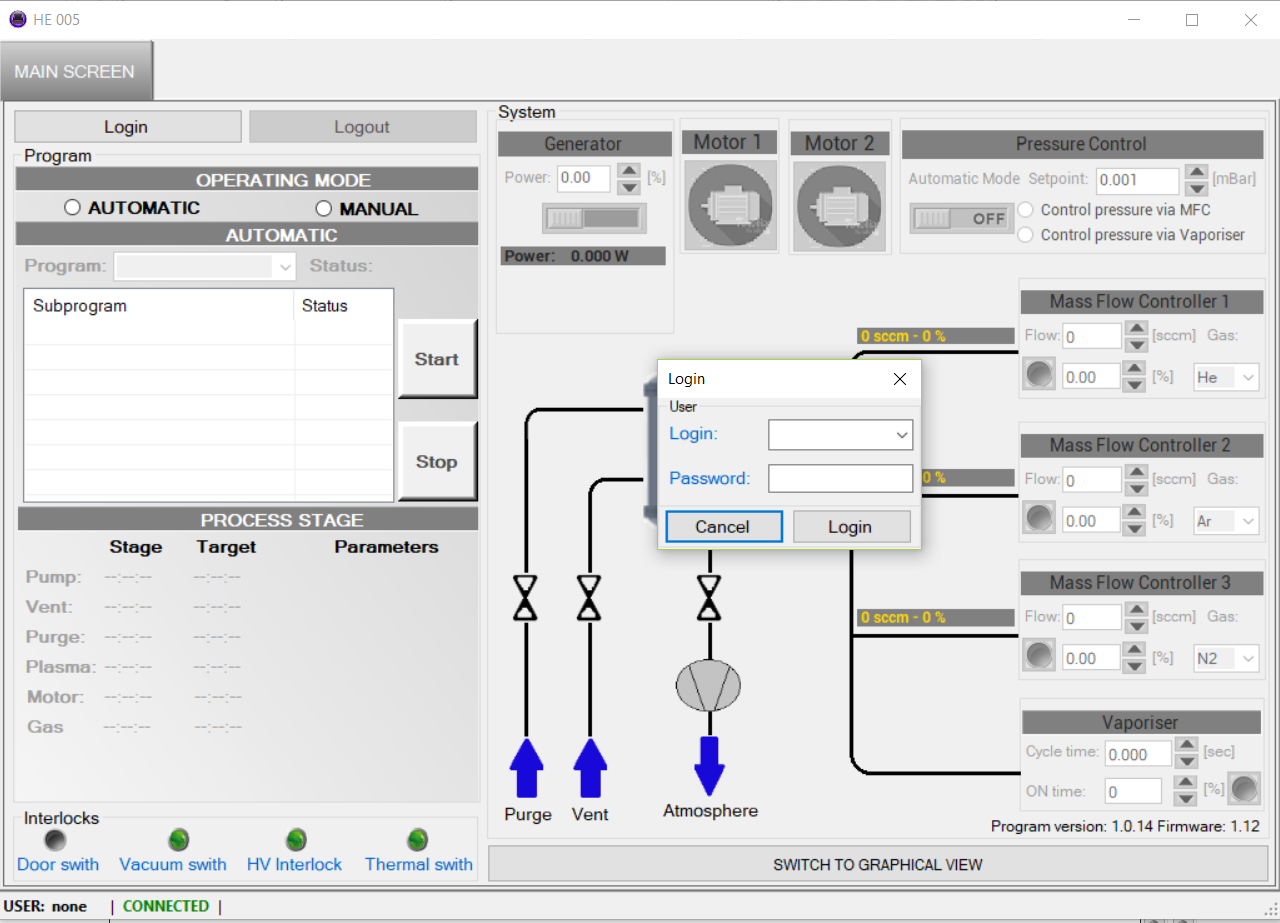
\includegraphics[width=0.8\textwidth]{Graphic/StartWorking/MainWindowWithLogin.png}	
	\caption{Main window with login}
	\label{main_window_with_login}
	\end{figure}
	\FloatBarrier

IMPORTANT: \\
In order to program could work correctly it need connection to controler of machine therefore user should check status of connection after logged to program. It was be as the image bellow - \textit{CONNECTED}. When notice something disturbing please see chapter \textit{Troubleshooting} in order to finda help to solve a problem.

	\begin{figure}[!h] 
	\centering 
\includegraphics[width=0.4\textwidth]{Graphic/StartWorking/ConnectionStatus.png}	
	\caption{Connection status}
	\label{connection_status}
	\end{figure}
	\FloatBarrier


\section {RUN PROGRAM}

When we want use machine to perform some process we should lunch automatic program. The program will perform step-by-step prepared operations. 

	\begin{figure}[!h] 
	\centering 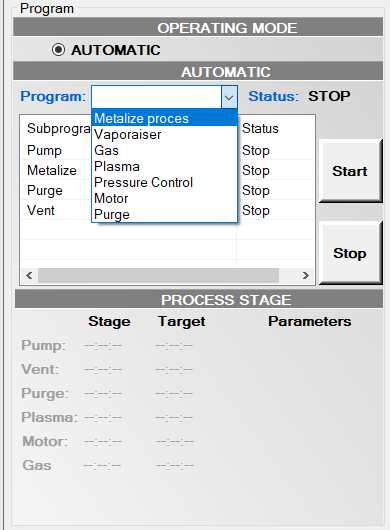
\includegraphics[width=0.4\textwidth]{Graphic/StartWorking/SelectProgram.png}	
	\caption{Select program}
	\label{select_program}
	\end{figure}
	\FloatBarrier

In order to launch a program please select one of defined programs and click \textit{Start}. Status of program should be changeg and set on one of the following states. When we want stopped program please click \textit{Stop}.

\begin{itemize}
	\item \textit{ Stop} - program is stopped. 
	\item \textit{ Run} - program is running. One of subprograms is working
	\item \textit{Done} - program has been finished sucessfully. All subprograms fisnished operation correctly.
	\item \textit{Error} - program stopped. One of subprograms reports error.
\end{itemize}

Each program consist of subprgorams. List of subprograms is showed below a program. After selected one of subprogram we can see which statge consist and what are the parameters. When program is running, subprogram can set one of bellow states:

\begin{itemize}
	\item \textit{ Stop} - subpprogram is stopped. 
	\item \textit{ Run} - subprogram is running.
	\item \textit{Done} - subprogram has been finished sucessfully.
	\item \textit{Error} - subprogram stopped. Some errors occured (which exactly we can check on \textit{Alert} tab).
\end{itemize}





